\documentclass[border=1cm,tikz]{standalone}

\usetikzlibrary{arrows.meta}

\definecolor{green}{rgb}{0.365, 0.592, 0.157}
\definecolor{darkblue}{rgb}{0.000, 0.275, 0.545}

\begin{document}

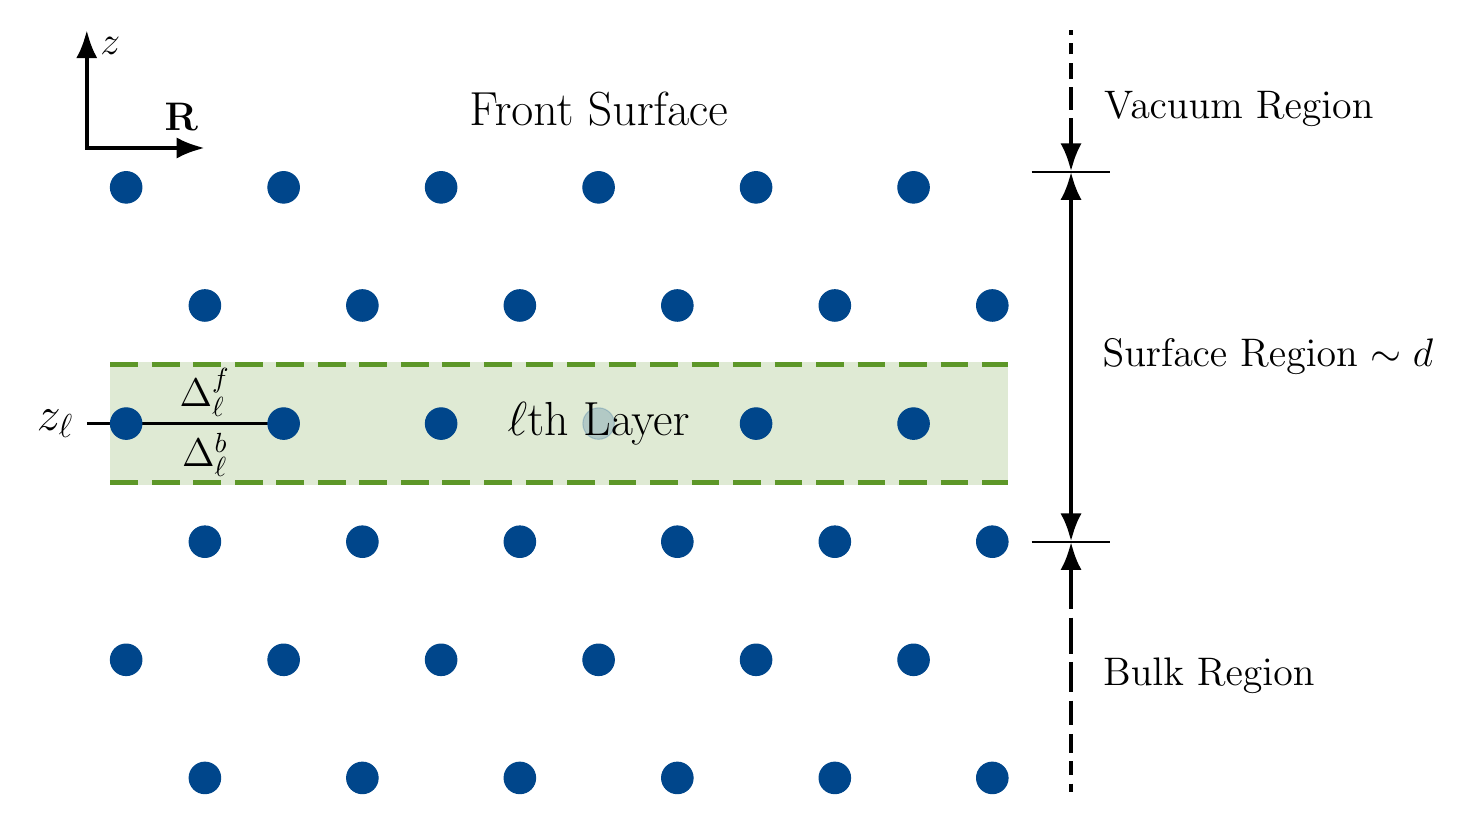
\begin{tikzpicture}

% right side markings
\draw[Latex-,dash pattern=on 10pt off 3pt on 8pt off 3pt on 6pt off 3pt on 4pt off 3pt on 2pt,ultra thick] (13,7.2) -- (13,9);
\node at (15.13,8) {\Large Vacuum Region};
\draw [thick] (12.5,7.2) -- (13.5,7.2);
\node at (15.5,4.85) {\Large Surface Region $\sim d$};
\draw [Latex-Latex,ultra thick] (13,2.5) -- (13,7.2);

\draw [thick] (12.5,2.5) -- (13.5,2.5);
\draw[Latex-,dash pattern=on 15pt off 3pt on 13pt off 3pt on 11pt off 3pt on 9pt off 3pt on 7pt off 3pt on 5pt off 3pt on 3pt off 3pt,ultra thick] (13,2.5) -- (13,-0.7);
\node at (14.75,0.8) {\Large Bulk Region};
% \draw[Latex-,dash pattern=on 15pt off 3pt on 5pt off 3pt on 3pt off 3pt,ultra thick] (13,-0.5) -- (13,1);
% \draw [thick] (12.5,-0.5) -- (13.5,-0.5);


% top and bottom text
\node at (7,8) {\LARGE Front Surface};
% \node at (7,-1.3) {\LARGE Back Surface};


% layer stuff
\draw [ultra thick,dash pattern=on 10pt off 5pt,green] (0.8,4.75) -- (12.2,4.75);
\fill [fill=green,fill opacity=0.2] (0.8,3.22) rectangle (12.2,4.78);
\draw [ultra thick,dash pattern=on 10pt off 5pt,green] (0.8,3.25) -- (12.2,3.25);
\node at (2,4.4) {\Large $\Delta^{f}_{\ell}$};
\node at (0.1,4) {\LARGE $z_{\ell}$};
\draw [thick] (0.5,4) -- (3,4);
\node at (2,3.6) {\Large $\Delta^{b}_{\ell}$};


% lattice zero row
\filldraw [darkblue] (2,-0.5)  circle (0.20);
\filldraw [darkblue] (4,-0.5)  circle (0.20);
\filldraw [darkblue] (6,-0.5)  circle (0.20);
\filldraw [darkblue] (8,-0.5)  circle (0.20);
\filldraw [darkblue] (10,-0.5) circle (0.20);
\filldraw [darkblue] (12,-0.5) circle (0.20);
% first row
\filldraw [darkblue] (1,1)    circle (0.20);
\filldraw [darkblue] (3,1)    circle (0.20);
\filldraw [darkblue] (5,1)    circle (0.20);
\filldraw [darkblue] (7,1)    circle (0.20);
\filldraw [darkblue] (9,1)    circle (0.20);
\filldraw [darkblue] (11,1)   circle (0.20);
% second row
\filldraw [darkblue] (2,2.5)  circle (0.20);
\filldraw [darkblue] (4,2.5)  circle (0.20);
\filldraw [darkblue] (6,2.5)  circle (0.20);
\filldraw [darkblue] (8,2.5)  circle (0.20);
\filldraw [darkblue] (10,2.5) circle (0.20);
\filldraw [darkblue] (12,2.5) circle (0.20);
% third row
\filldraw [darkblue] (1,4)    circle (0.20);
\filldraw [darkblue] (3,4)    circle (0.20);
\filldraw [darkblue] (5,4)    circle (0.20);
\filldraw [darkblue,opacity=0.2] (7,4)    circle (0.20);
\filldraw [darkblue] (9,4)    circle (0.20);
\filldraw [darkblue] (11,4)   circle (0.20);
% fourth row
\filldraw [darkblue] (2,5.5)  circle (0.20);
\filldraw [darkblue] (4,5.5)  circle (0.20);
\filldraw [darkblue] (6,5.5)  circle (0.20);
\filldraw [darkblue] (8,5.5)  circle (0.20);
\filldraw [darkblue] (10,5.5) circle (0.20);
\filldraw [darkblue] (12,5.5) circle (0.20);
% fifth row
\filldraw [darkblue] (1,7)    circle (0.20);
\filldraw [darkblue] (3,7)    circle (0.20);
\filldraw [darkblue] (5,7)    circle (0.20);
\filldraw [darkblue] (7,7)    circle (0.20);
\filldraw [darkblue] (9,7)    circle (0.20);
\filldraw [darkblue] (11,7)   circle (0.20);


% surprise motherfucker!
\node at (7,4) {\LARGE $\ell$th Layer};


% axes
\draw [Latex-Latex,ultra thick] (2,7.5) -- (0.5,7.5) -- (0.5,9);
\node at (0.8,8.8) {\Large $z$};
\node at (1.7,7.9) {\Large $\mathbf{R}$};
\end{tikzpicture}

\end{document}
